\chapter{Approach and Methodology}
\section{Overview}
After understanding the scope of improvement in the existing analog measurement signals processing methodology,
a new approach is worked out and implemented within the Low Voltage MTS setup.
The new approach involves some action items that are needed to be completed at a certain chronology.
The sequence of action items is depicted in \cref{fig:flowchart}.
\Cref{sec:dataproc} describes the data processing concepts that are derived for processing analog measurements in MicroMoPS. 
\Cref{sec:identification} describes the identification of boards in the stress test environment and preparation of board related information in the MoPS web server.
\Cref{sec:host application} describes the automated procedure of processing analog measurements regardless of the board combinations.
\begin{figure}[hbt]
		\centering
		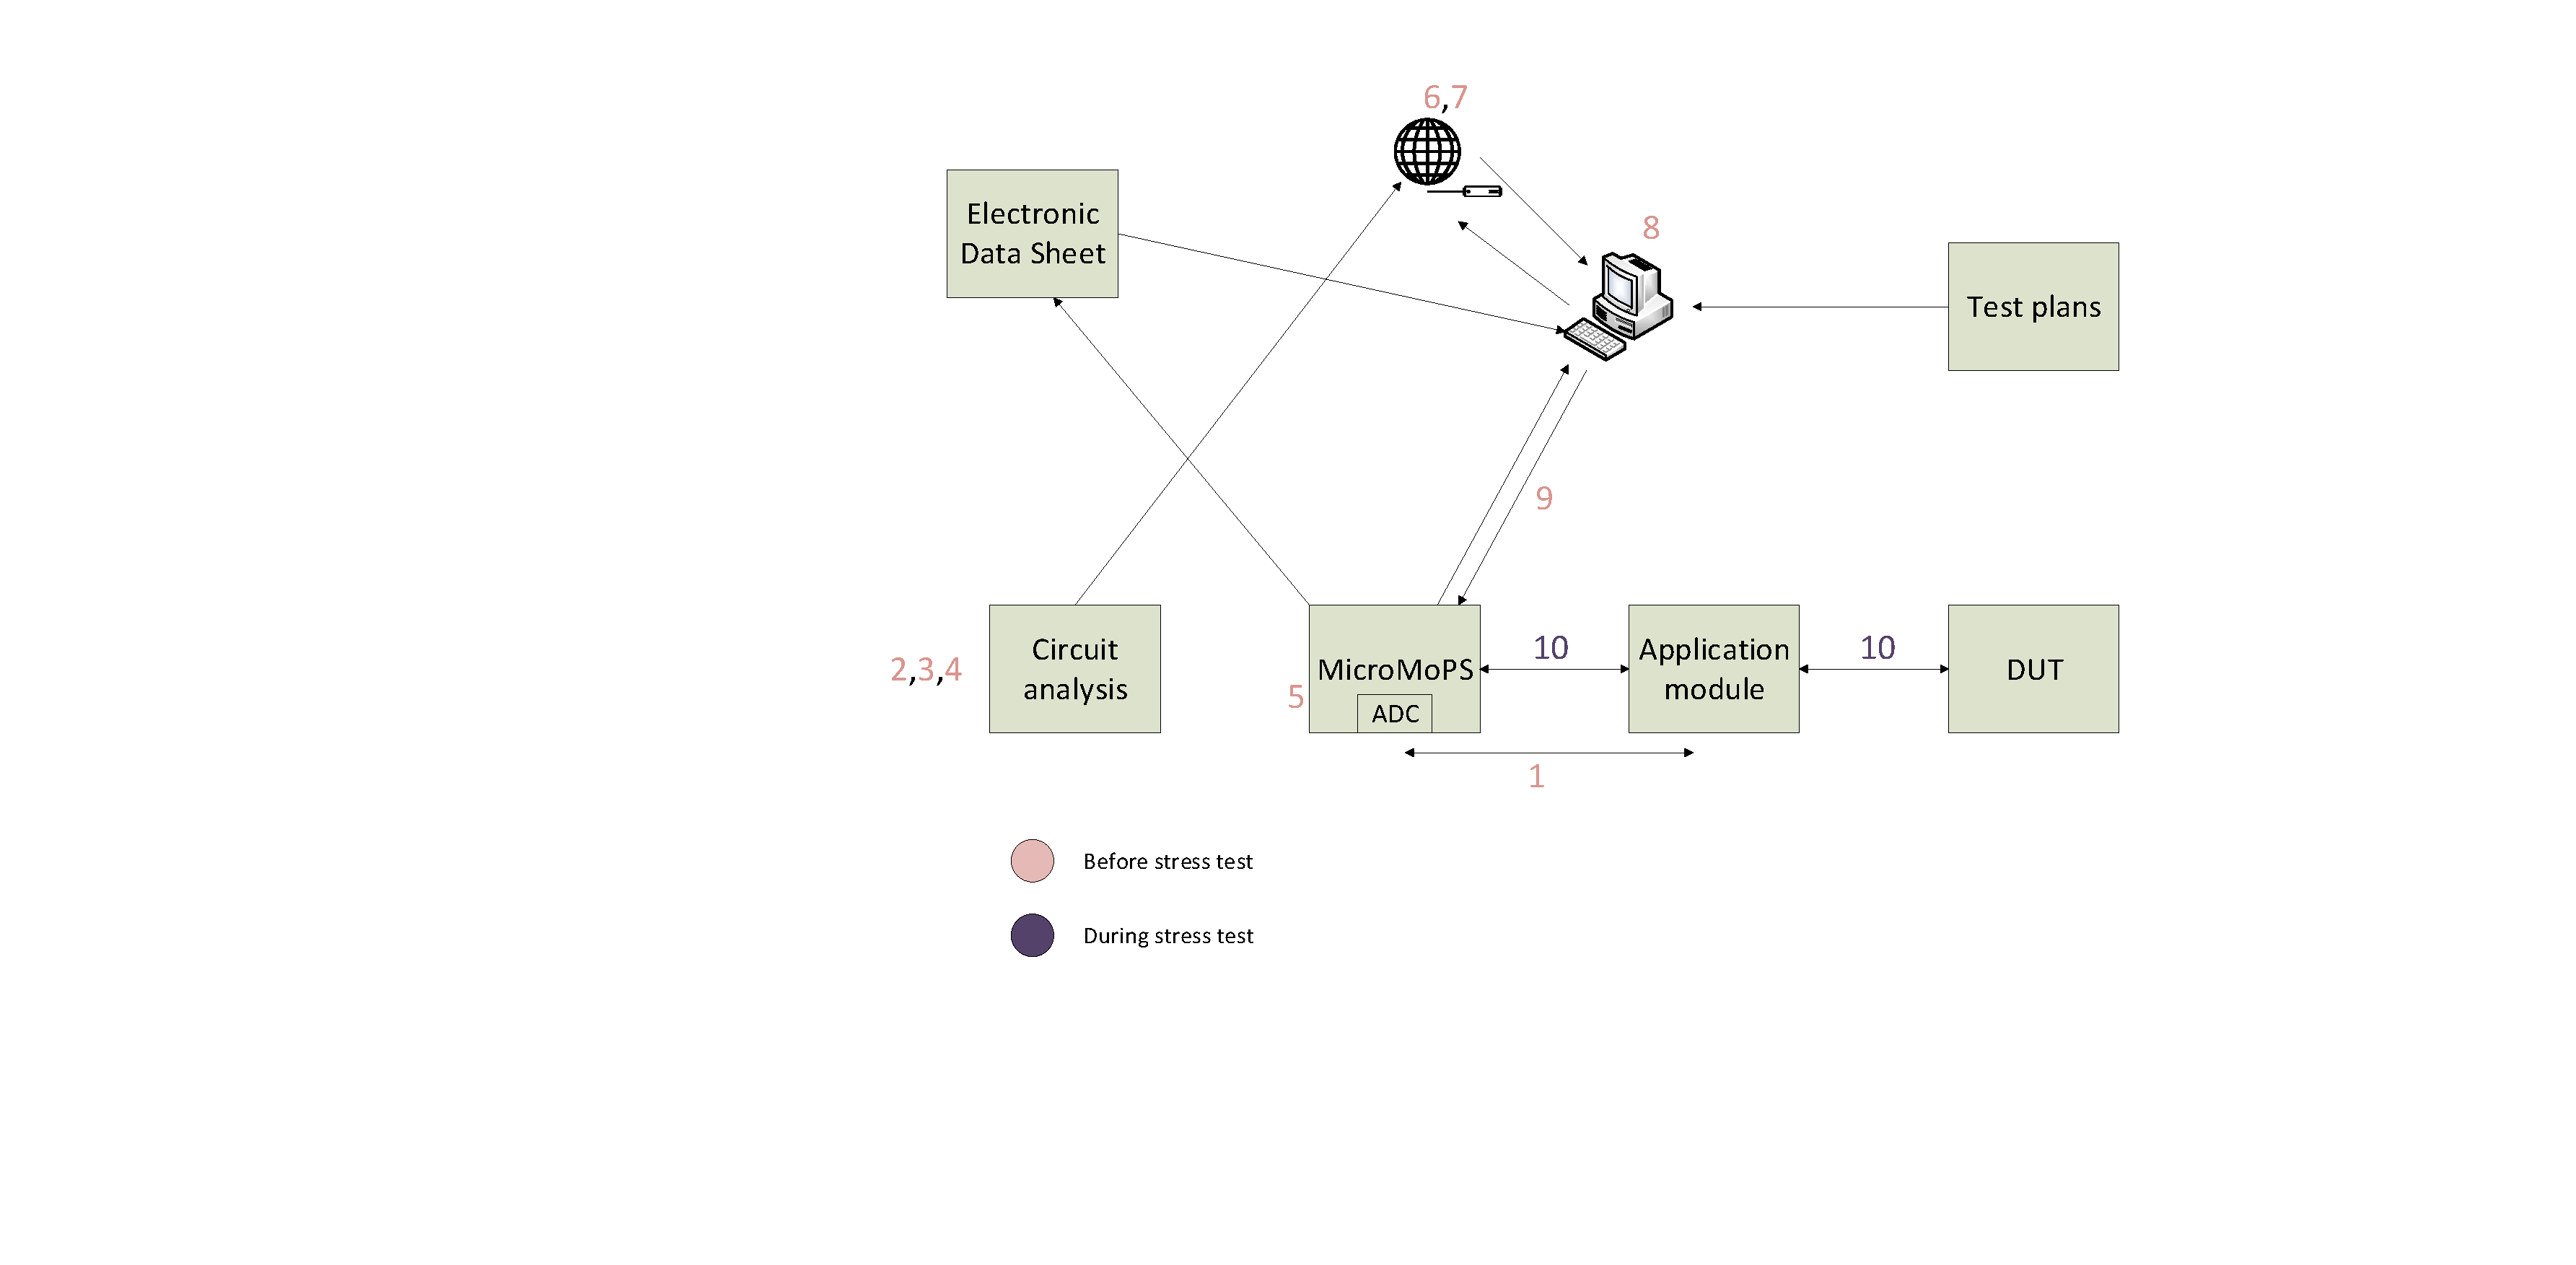
\includegraphics[trim=540 150 0 0, clip, width=195mm]{images/Approach_and_methodology.pdf}
		\caption{Enhancements.}
		\label{fig:flowchart}
\end{figure} 

\section{Derive data processing concepts for stress test environment}\label{sec:dataproc}

\subsection{Acquiring a signal model}\label{sec:SM}	
	\begin{figure}
	\centering
	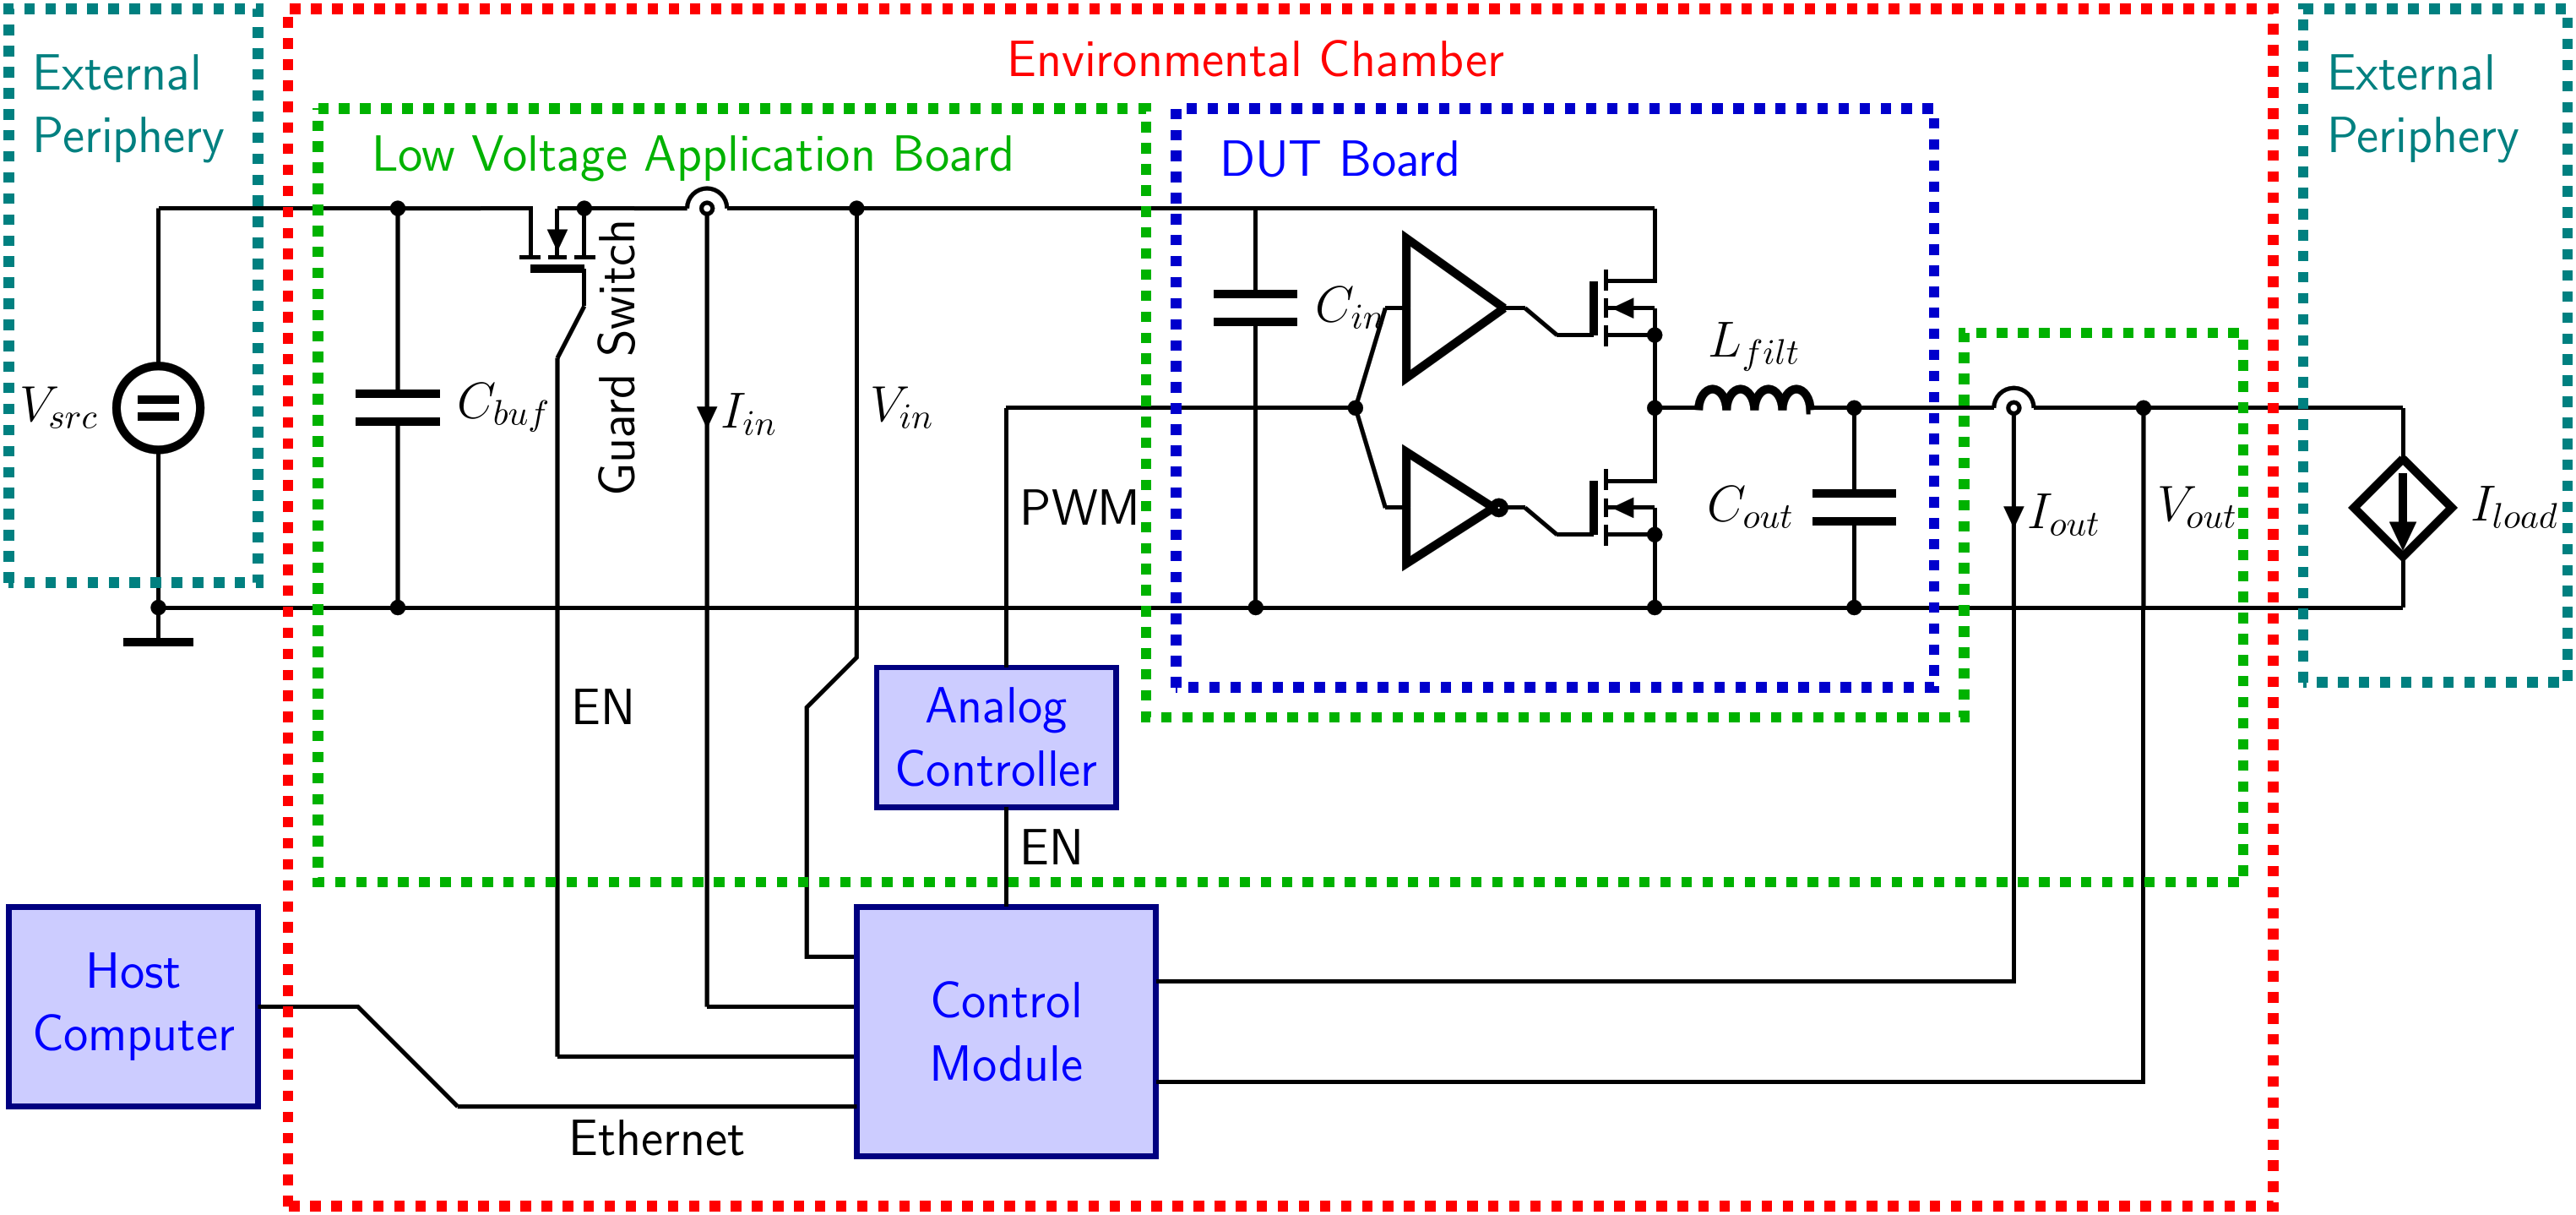
\includegraphics[trim=0 0 0 0, clip, width=\textwidth]{images/LV_module_2.png}
	\caption{Low Voltage Modular test system.}
	\label{fig:LVMTS}
	\end{figure}

In the modular stress test environment, the application module is used for submitting stresses on DUT. 
The used application module involves its own application specific characteristic circuitry.
In this work, since it is the Low-Voltage stress test system that is used, the discrete power transistors are submitted to \emph{power cycling} (~\cite{Sleik2016}, p.2) test. 
This is a test in which \acrshort{DUT}s are pulled to their extreme operating conditions by introducing them into various scenarios. %DUTs are heated to reach temperature between \SIlist{85;125}{\celsius} for consumer devices, \SI{150}{\celsius} for automotive devices and are supplied with supply voltage that is set to maximum level which still complies the data sheet specificiation of DUT. Intermittent loads are submitted to DUTs which toggle between a high load of \SI{100}{\percent} that nearly reaching DUTs to their maximum operating temperature and a low load of \SI{10}{\percent}.} 
Further, in response to a "power cycling" test, certain \acrshort{MTS} parameters are measured. %such as Iin, Iout, Vin, Vout, Tcase, Idrv, Vdrv, Imon and Tmon(see Section \cref{Channels}).
These parameters of the Low Voltage MTS are recorded based on the control logic implemented by a PI controller at BuckMoPS (\cref{sec:BuckMoPS}). 
As a result, the measurement signals are automatically monitored by a control module throughout the entire test. 
These measurement signals go through conditioning before reaching the ADC, as explained in \cref{sec:asc}. 
To obtain the real time efficient scaling mechanism for MicroMoPS, the path that the measurement signals traverse from the source of the signal conditioning circuits to the source of the analog-to-digital converter of the control module as shown in \cref{fig:Signal model}, are analysed in this work. 
The path that the measurement signals travel consist of the measurement circuits that are associated with acquisition of measurements. 
Further, the signal path information is obtained by following the hardware schematics of MicroMoPS and application module. 
The values of every active and passive device that are present in the measurement circuitry is important to know because it helps in obtaining scaling factor associated parameters which are specific to the respective type of measurements.
\begin{figure}[htb]
	\centering
	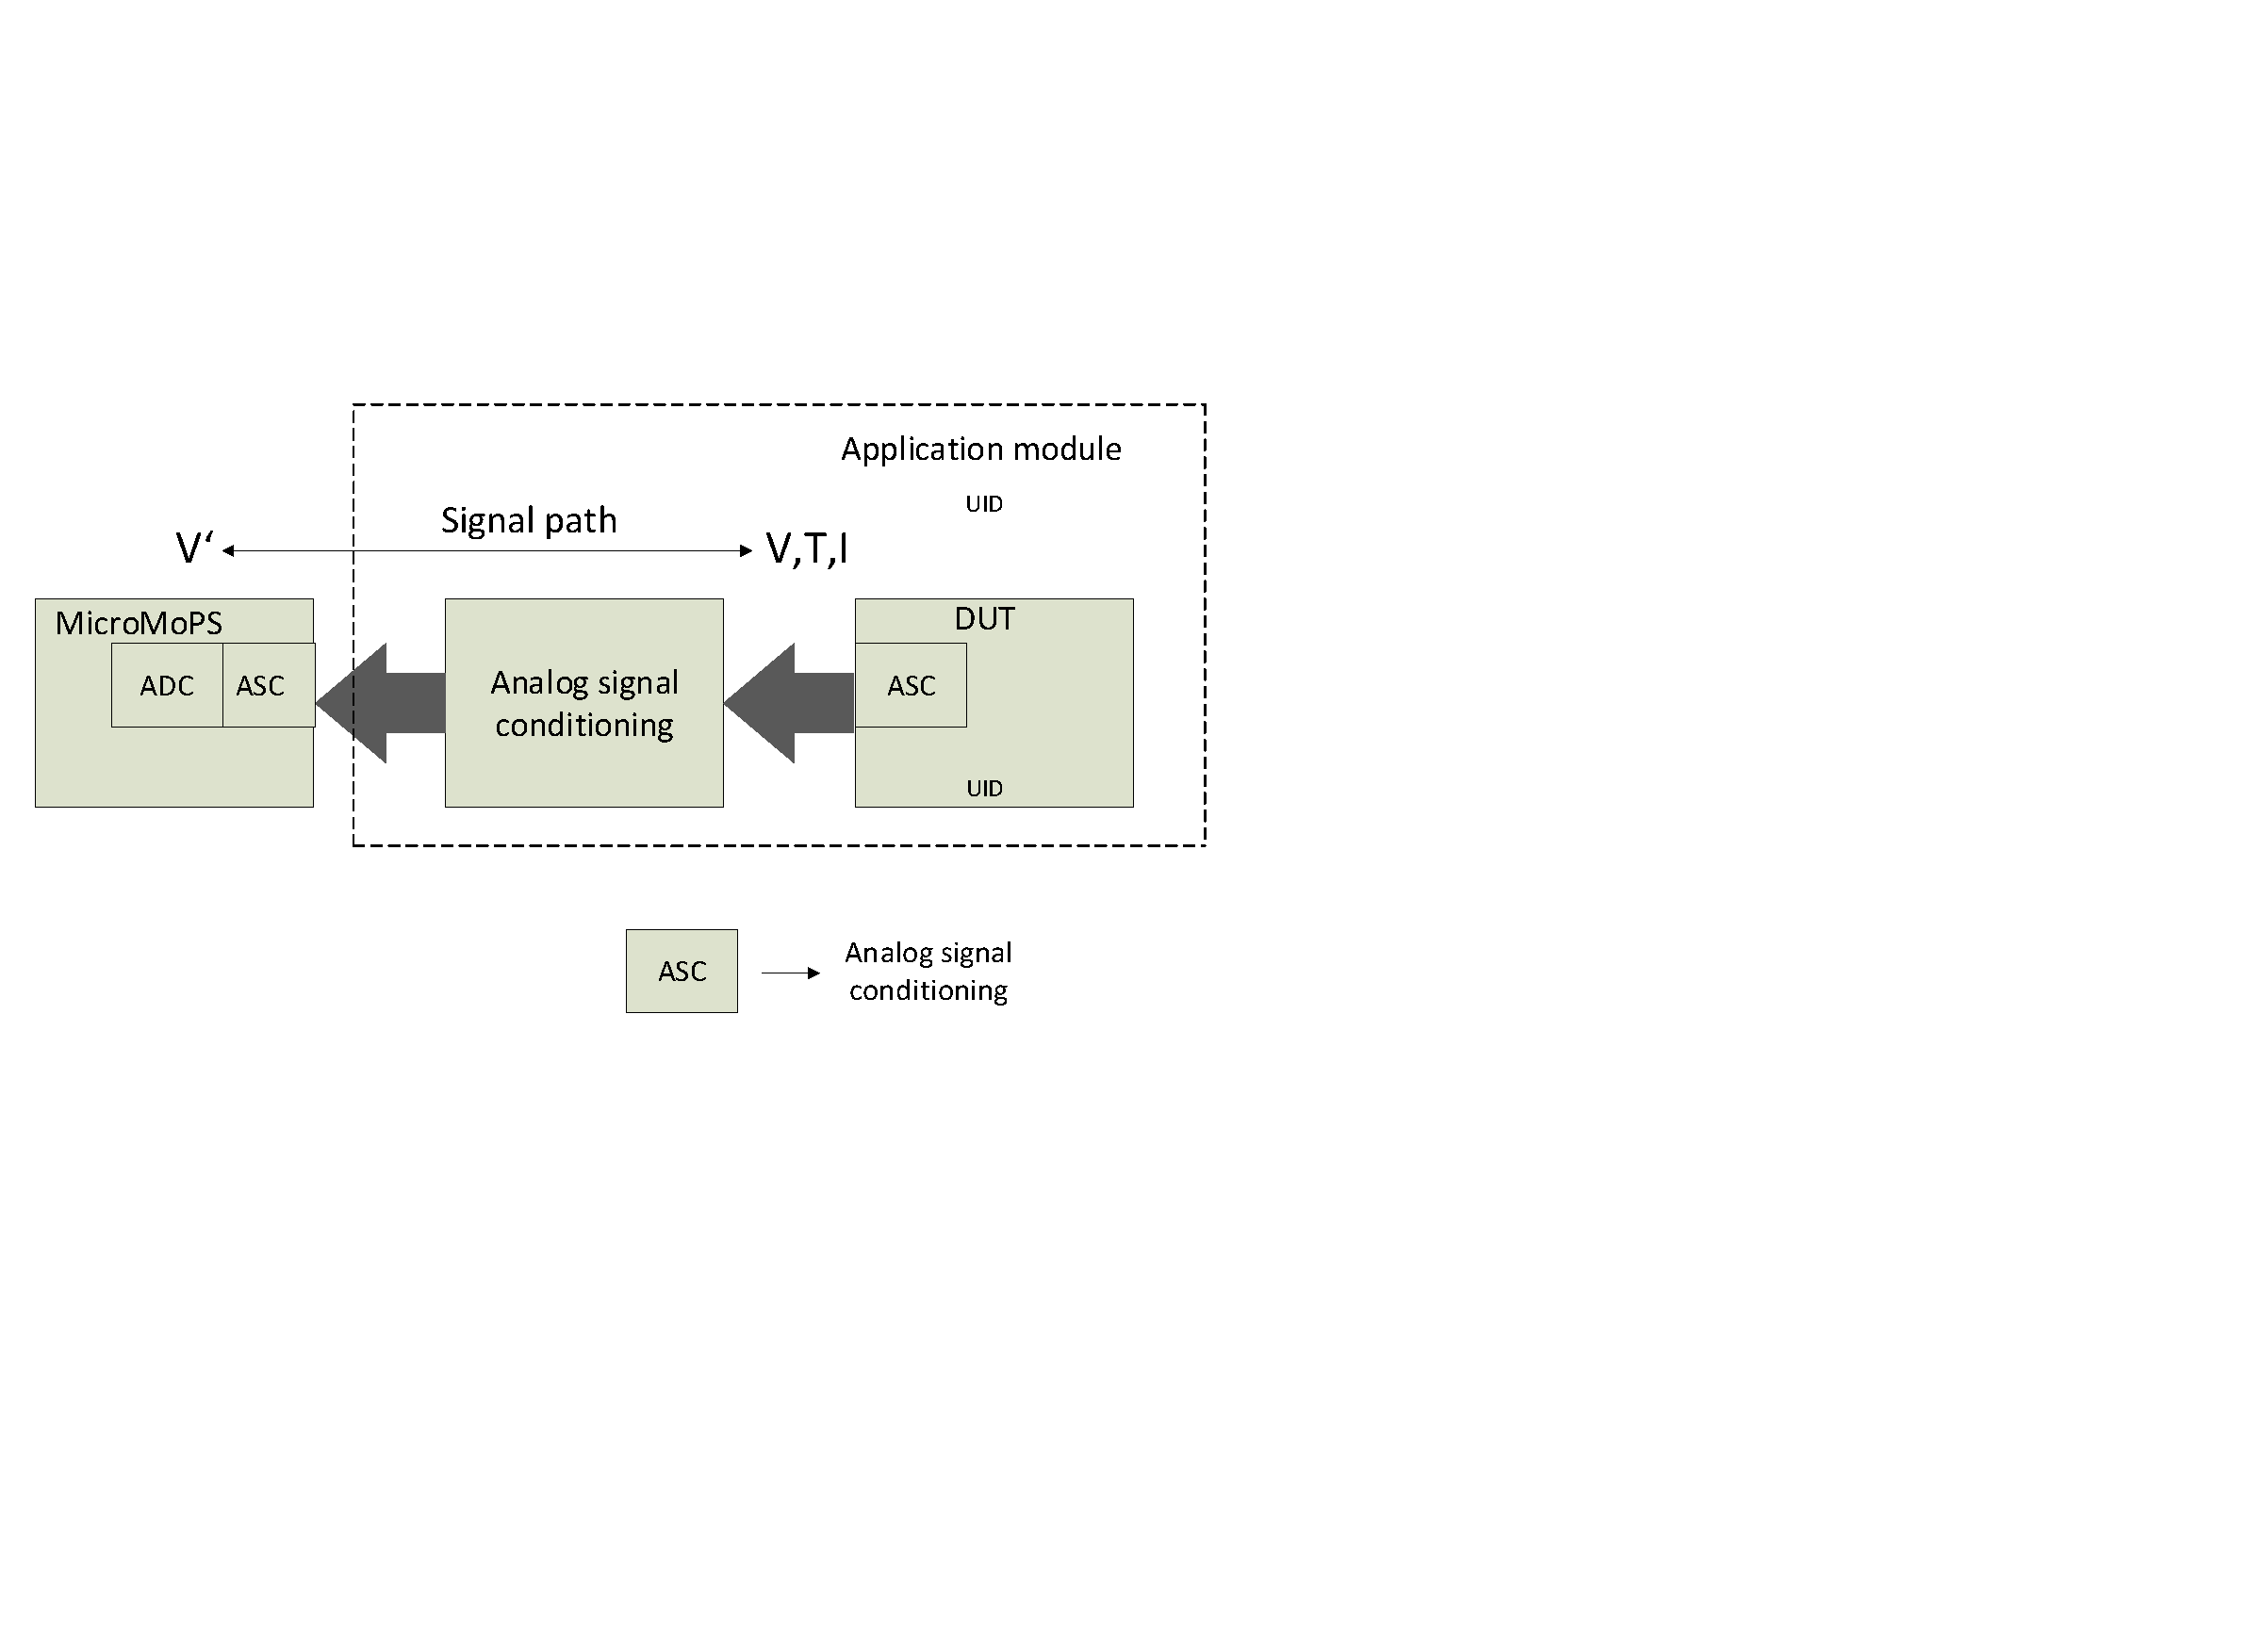
\includegraphics[trim=0 400 400 150, clip, width=\textwidth]{images/Signalmodel.pdf}
	\caption{Signal path of measurement data acquisition.}
	\label{fig:Signal model}
\end{figure}

The series resistors (R1, R3), differential operational amplifier and the standard voltage divider circuit (R2, R4, R5 and R6) conventions (see \cref{fig:Conditioning}) are part of the analog signal conditioning circuit as described in \cref{sec:asc}. 
They are defined by Hardware designers at KAI to appropriately attenuate the electrical signals into MicroMoPS operating voltage range from \SIrange{0}{3}{\volt}.
The defined circuit component values are listed as shown in \cref{Table1}.

%Assumptions of circuit components
%\vspace{2cm}
%\centering

\begin{table}
	\centering
	\caption{Component values}
	\label{Table1}
	\begin{tabular}{ |p{3cm}||p{1.5cm}|p{1.5cm}|p{1.2cm}|p{1cm}|p{1.2cm}|p{1cm}|  }
	\hline
	\textbf{Signal}   & \textbf{R1}    &\textbf{R2}   &\textbf{R3}   &\textbf{R4}   &\textbf{R5}   &\textbf{R6}\\
	\hline
	Iin   &\SI{18}{\kilo\ohm}   &60k\si{\ohm}   &18k\si{\ohm}   &60k\si{\ohm}   &15k\si{\ohm}   &15k\si{\ohm}\\
	Iout   &27k\si{\ohm}    &60k\si{\ohm}   &27k\si{\ohm}   &60k\si{\ohm}   &75k\si{\ohm}   &75k\si{\ohm}\\
	Vin   &26.9k\si{\ohm}    &4.02K\si{\ohm}   &26.9k\si{\ohm}   &2k\si{\ohm}   &NP   &NP\\
	Vout   &6.7k\si{\ohm}    &4.02K\si{\ohm}   &6.7k\si{\ohm}   &2k\si{\ohm}   &NP   &NP\\  	
	Imon   &2k\si{\ohm}    &2k\si{\ohm}   &2k\si{\ohm}   &2k\si{\ohm}   &4.02k\si{\ohm}   &2k\si{\ohm}\\
	\hline
	\end{tabular}
	\label{table:circuit_components}
\end{table}

		\subsection{Derive transfer characteristics to find scaling parameters.}\label{sec:Transfer Function}
		After obtaining a signal model which provides information about the measurement circuit of the Low Voltage stress test environment, the circuits that are present in the signal path are analysed to derive the transfer function between the source of the signal conditioning circuits and the source of the analog-to-digital converter of the MicroMoPS. 
		Derivation of the transfer function is done using one of the standard circuit analysis techniques (e.g. Superposition theorem).  
Measurements such as \gls{Vin}, \gls{Vout}, \gls{Iin}, \gls{Imon} and \gls{Iout} with differential amplifier circuits (see \cref{sec:asc}) are analysed using Superposition theorem. 
Using the Superposition theorem, three equations of input/output relations are obtained from which, the transfer function is derived. 
The derived transfer function is further simplified. The steps that are involved in deriving the transfer function are as follows: 
%Transfer function steps and simplification

\begin{enumerate}
  \centering
\item $V_1$ and $V_2$ are shorted.\\
	\vspace{4mm}
	\hspace{30mm}
	  %$V_01$ = $V_ref$.\[ \cfrac{V_ref}{b} \] 
	  	$V_{o1}$ = $V_{ref}$ .$\dfrac{R_3||R_4}{R_6 + R_3||R_4}$.$\left(1 + \dfrac{R_2}{R_1 + R_5}\right)$
\item $V_1$ and $V_{ref}$ are shorted.\\
	\vspace{4mm}
	\hspace{28mm}
	  %$V_01$ = $V_ref$.\[ \cfrac{V_ref}{b} \] 
	  $V_{o2}$ = $V_{2}$ .$\dfrac{R_4||R_6}{R_3 + R_4||R_6}$.$\left(1 + \dfrac{R_2}{R_1 + R_5}\right)$
\item $V_2$ and $V_{ref}$ are shorted.\\
	\vspace{4mm}
	\hspace{-9mm}
	  %$V_01$ = $V_ref$.\[ \cfrac{V_ref}{b} \] 
	  $V_{o3}$ = $V_{1}$ .$\left(-\dfrac{R_2}{R_1}\right)$
\end{enumerate}

\begin{flushleft}
\hspace{-9mm}
$V_{out}$ results in $V_{out}$ = $V_{o1}$ + $V_{o2}$ + $V_{o3}$, which equals the expression of nodal analysis, i.e.

\hspace{-9mm}
$V_{out}$ = $\dfrac{R_3R_4R_6}{R_3R_4 + R_3R_6 + R_4R_6}$$\left(\dfrac{R_2}{R_1 + R_5} + \dfrac{V_{ref}}{R_6}\right)$$\left(1 + \dfrac{R_2}{R_1} + \dfrac{R_2}{R_5}\right)$ - $\dfrac{R_2}{R_1}V_1$.

\hspace{-9mm}
The resistor relations assumptions are applied:


\hspace{-9mm}
${R_1}$ = ${R_3}$\\
\hspace{-9mm}
${R_2}$ = ${R_4}$\\
\hspace{-9mm}
${R_5}$ = ${R_6}$

\hspace{-9mm}
This further simplifies the $V_{out}$ equation to

\hspace{-9mm}
$V_{out}$ = $\dfrac{R_2}{R_1}$($V_{1}$ - $V_{2}$) + $\dfrac{R_2}{R_5}$$V_{ref}$, \hspace{9mm} where ($V_{1}$ - $V_{2}$) = $V_{in}$ 
\end{flushleft}

\hspace{-10mm}Further, the information of MicroMoPS' voltage range and resistor values as described in \cref{sec:Channels} and \cref{table:circuit_components}, respectively, are specific to measurement channels. These values are plugged into the derived transfer function to 
obtain the measurement range of the voltage or current or temperature signal before 
conditioning. The algebraic method of performing the above explained calculation is 
demonstrated by considering a '\acrshort{Vin}' measurement parameter's signal path as an example.	

\hspace{-10mm}
For '$V_{in}$' measurement parameter the $V_{out}$ equation simplifies to,
%algebraic expression using example

\begin{equation}
V_{out} = \dfrac{R_2}{R_1}.V_{in}, 
\label{eq:Vout}
\end{equation}

\hspace{-10mm}
To find '$V_{in}$' measurement range, the maximum voltage condition of MicroMoPS is considered and the values corresponding to $V_{in}$ are put to \cref{eq:Vout},

\hspace{-9mm}3V = $\dfrac{4.02\kilo}{26.9\kilo}V_{imax}$,\\

\hspace{-9mm}-> $V_{imax}$ = 20.17500 V

\hspace{-9mm}Similarly, minimum voltage condition corresponding to $V_{in}$ becomes,

\hspace{-9mm}0V = $\dfrac{4.02\kilo}{26.9\kilo}V_{imin}$, \\

\hspace{-9mm}-> $V_{imin}$ = 0 V

\hspace{-9mm}Likewise, the measurement range of the signal at source is found for all the measurement parameters. They are listed in \cref{Table2}.
%table

\begin{table}[ht]
	\centering
	\caption{Measurements range}
	\label{Table2}
	\begin{tabular}{ |p{3cm}||p{1.5cm}|p{1.5cm}| }
	\hline
	\textbf{Signals}   & \textbf{min}    &\textbf{max} \\
	Iin   &-5A   &10A \\
	Iout   &-5A    &70A\\
	Vin   &0V    &20.175V\\
	Vout   &0V    &5.020V\\  	
	Imon   &0V   &0.305V\\
	\hline
	\end{tabular}
\end{table}

\hspace{-9mm}Also, the measurement range of other parameters are found by either simple nodal analysis method or they are present in hardware schematics of application module. 

\hspace{-9mm}Using the obtained measurement ranges, the measurement specific linear equation fitting scaling parameters are found out. 
The algebraic method of finding out scaling parameters is explained by reconsidering the same measurement parameter, i.e., \acrshort{Vin}. 
%algebraic expresion

\hspace{-9mm}Linear scaling function is given by \\ 
y = k*x + d,      \\
\hspace{9mm} where, y = analog value, \\
\hspace{9mm} k = scaling factor, \\
\hspace{9mm} x = digital representation of analog measurement, \\
\hspace{9mm} d = offset

\hspace{-9mm}For maximum voltage condition of Vin, the digital value is 4095	 (12 bit resolution, see \cref{sec:DAQ}), the analog value is the maximum \acrshort{Vin} measurement from the \cref{Table2}\\

\begin{equation}
20.175 = k(4095) + d
\label{eq:Vmax}
\end{equation}

%\hspace{-9mm}-> 20.175 = k(4095) + d ............(3)

\hspace{-9mm}Similarly, for minimum voltage condition of Vin, the digital value is 0, the analog value is the minimum \acrshort{Vin} measurement from the \cref{Table2}

\begin{equation}
0 = k(0) + d
\label{eq:Vmin}
\end{equation}

%\hspace{-9mm}-> 0 = k(0) + d ............(4)

\hspace{-5mm}Solving \cref{eq:Vmax} and \cref{eq:Vmin} using substitution method, the values of scaling parameters that are associated to \acrshort{Vin} measurement parameter are obtained as below.\\

\hspace{-3.5mm}k = 0.0049267399267399,\\
\hspace{3mm}d = 0

From the obtained scaling parameters 'k' and 'd', it is evident that the found scaling parameters could be used for processing the digitized stress measurements to original signal value (signal before conditioning) but not to MicroMoPS specific voltage range. 
Therefore, the linear equation is further improved by considering additional parameters in the scaling function.   

\subsection{Find a linear scaling function from obtained scaling parameters.}\label{sec:linear function}
The improvement of the linear scaling function as discussed in the previous section is achieved by considering the changing factor inside the linear scaling function. 
The mentioned changing factor influences in determining the appropriate scaling values that precisely process analog measurements into MicroMoPS specific voltage values. It is given by,

%$V_01$ = $V_ref$.\[ \cfrac{V_ref}{b} \]

%y = \[
%		\left[{$\left(k - \dfrac{V_{max}-V'_{max}}{4096}\right)$*x + d}\right]$  V\\ 
%	  \]

\[ y =  
 \left[\left(k - \frac{V_{max}-V'_{max}} {4096}\right)*x + d \right] V
\] 

If the measurement parameter is temperature or voltage signal then, the improved linear scaling equation is as shown below,

%y = $\left[k - \dfrac{(I|T)_{max}*g-V'_{max}}{4096}\right]$*x + d \ldots V\\ 

\[ y = 
 \left[\left(k - \frac{(I|T)_{max}*g-V'_{max}} {4096}\right)*x + d \right] V
\] 

where, 'I' is the current measurement signal and 'T' is the temperature measurement signal.
%equation
	The changing factor represents the change in maximum value of the original (V/T/I) signal and the maximum voltage of the attenuated signal (V') as represented in the \cref{fig:Signal model}. 
	The value '4096' in the equation represents the factor that contributes in the occurring change. 
	Finally, the transconductance parameter 'g' does the necessary conversion of temperature or current signals into respective voltage values (V').

For the measurement parameter \gls{Tcase}~\cite{Sleik2018a}, since it is the resistive sensor that is fed directly on to ADC of the MicroMoPS instead of a differential amplifier, the scaling parameters for $T_{case}$ are found in a differently instead of deriving transfer function.
The DUT board is let to go into temperature ranging between \SIlist{-55;37}{\celsius}.
Consequently, the corresponding voltage that is generated because of voltage amplification for every different board temperature is measured. 
Using the generated voltage information, scaling parameters ('k', 'd') and transconductance parameter ('g') are found. 
Scaling parameters of all the measurements and the measurements respective units are listed in Table 4.3.

\begin{table}[ht]
	\centering
	\label{table:Table3}
	\caption{Measurement parameters}
\begin{tabular}{ |p{3cm}||p{3cm}|p{1.5cm}|p{1.5cm}|}
 \hline
 \multicolumn{4}{|c|}{Scaling parameters associated to Measurements} \\
 \hline
 \textbf{Signals}   & \textbf{k}    &\textbf{d}  &\textbf{Units}\\
Iin   &0.000732601   &0.0 &A\\
Iout   &0.000732601   &0.0 &A\\
Vin   &0.000363   &0.0 &V\\
Vout   &0.000363    &0.0 &V\\  	
Imon   &0.000732601   &0.0 &A\\
Vdrv   &0.000732609   &0.0 &V\\
Idrv   &0.000733   &0.0 &A\\
Imon   &0.000732601   &-1.5 &V\\
Tcase   &0.000734056   &0.0 &C\\
Vswh   &0.000732601   &0.0 &V\\
Tmon   &0.000732601   &0.0 &V\\
Aux1   &0.000732601   &-1.5 &V\\
Aux2   &0.000732601   &0.0 &V\\
 \hline
\end{tabular}
\end{table}

Supposedly, if the stress test is of any application other than Low Voltage MTS, then the respective test application specific processing parameters such as \textbf{k}, \textbf{d}, \textbf{${V_{max}}$}, \textbf{${V'_{max}}$} and \textbf{g} are the only information that are needed to precisely process the analog measurements.

\subsection{Extended scaling mechanism.}\label{sec:RPN}   
Reverse Polish Notation (RPN) is a memory-efficient method that could be used in performing the scaling function. 
The working principle of RPN is explained by considering the scaling function of one of the channels (see \cref{sec:Channels}) of MicroMoPS as an example.

For example, the Scaling function of channel sync[0][0]B is (d/4096)*3 where d is a digital value. \acrshort{RPN} method of computing this scaling function is:      

\begin{itemize}[label={}]
\item \textbf{Step1:} Convert the scaling function into a string i.e "d 4096 / 3 *". For the sake of understanding, if d is given a digital value of 2048 then, the RPN notation becomes "2048 4096 / 3 *". 
\item \textbf{Step2:} Push 2048 onto Lua stack.
\item \textbf{Step3:} Push 4096 onto Lua stack.
\item \textbf{Step4:} Pop from lua stack twice, use the operator '/' to calculate 2048/4096 and push the result i.e. 0.5 onto Lua stack. 
\item \textbf{Step5:} Push 3 onto Lua stack.
\item \textbf{Step6:} Pop from Lua stack twice, use operator '*' to calculate 0.5*3 and push the result i.e 1.5 onto Lua stack.

This way, the scaling is performed for every communication channel of MicroMoPS using RPN.
\end{itemize}

\section{Identify the boards and prepare \glspl{LUT} in web server}\label{sec:identification}

\subsection{Board UID extraction.}\label{sec:identify}
The starting point of the Low-Voltage MTS setup is the operation of the test sequence in MicroMoPS.
The test sequence is executed by the central control entity i.e \acrshort{SAM} as a test plan.
Before, the DUT is subjected to \emph{power cycling} (see \cref{sec:MTS}), the extraction of \acrshort{UID} of the boards is an important step.
It is considered important because it helps in meeting one of the objectives of this work, which is to automate the processing of analog measurements in MicroMoPS.
Identification of the UID of the application module and DUT is done by pursuing I2C communication between the control module and a UID provider chip (see \cref{comm}) of application module and DUT, respectively.
To achieve I2C communication, the concerned functional pins of the control module are used and standard steps of the communication procedure are followed (see \cref{sec:IIC}).
Thereby, the UID of MicroMoPS itself is read from a register.
\subsection{Prepare board ID database in MoPS web server.}\label{sec:web server}
The board \glspl{UID} which are obtained from the MicroMoPS are communicated through Ethernet to its host application system called SAM.
Proactively, every board combination which corresponds to a particular type of stress test along with the board \glspl{UID} are stored as a lookup database as shown in the \cref{lst:boards}, in MoPS web server (see \cref{sec:CORE}). 

%\begin{listing}[htp]
%	\inputminted[frame=single]{JSON}{src/boards.json}
%	\caption{MoPS Boards}
%	\label{lst:boards}
%\end{listing}

\lstinputlisting[frame=single, label=lst:boards, caption=MoPS Boards, firstnumber=1]{src/boards.json}

\subsection{Store the scaling values meaningfully in MoPS web server database.}\label{sec:database}
Based on the communication channels' configuration information provided in the EDS and mathematically obtained scaling parameters for each of these communi	cation channels, a \gls{LUT} is created as shown in the \cref{lst:scaling}, in the \gls{MoPS} web server.
The created \gls{LUT} contains the scaling related information.  

%\begin{listing}[htp]
%	\inputminted[frame=single]{JSON}{src/scaling.json}
%	\caption{MoPS Scaling example}
%	\label{lst:scaling}
%\end{listing}

\lstinputlisting[frame=single, label=lst:scaling, caption=MoPS Scaling example, firstnumber=1]{src/scaling.json}

\subsection{Send UIDs before MicroMoPS enters into real-time mode.}\label{sec:UID}
The extracted board \glspl{UID} along with their directional pins are embedded as a single string and communicated as a payload to \acrshort{SAM} using Ethernet communication. 
The board UIDs communication is ensured to take place before the firmware enters into the main loop. 
The reason for the UIDs communication before main loop is to avoid redundant communication of UIDs and also to keep short the time that elapses from entering into main loop till the test pattern starts to execute in MicroMoPS. The time at which the control module enters inside an infinite loop is considered as an entrance towards the real-time mode of this stress test environment. In the real-time mode, the role of the control module is to endlessly perform tasks that are associated with the stress test system.
 
\section{Resolve UIDs in SAM and send the scaling values to MicroMoPS}\label{sec:host application}

\subsection{Resolution of UIDs in SAM}\label{sec:uidResolution}
Before the control module enters into a real-time mode the \acrshort{EDS} is generated. SAM reads the latest EDS from the MicroMoPS firmware project. 
The EDS that is read by SAM is uploaded to the MoPS web server (see \cref{sec:CORE}). 
SAM becomes functional when test engineers at KAI start to perform the application specific stress test. 
As soon as SAM starts running, it downloads \glspl{LUT} associated to scaling and boards (see \cref{fig:combination}) that are created in MoPS web server. 
The \glspl{LUT} associated to scaling and boards  are as shown in \cref{lst:scaling} and \cref{lst:boards} respectively. 
The \glspl{LUT} associated to scaling and boards together help the SAM to automate the scaling mechanism regardless of the type of stress tests that are performed. Test plans are created by test engineers and are loaded to SAM.


The flow at which the resolution of board UIDs and the communication of associated channel and scaling related parameters to MicroMoPS is depicted in \cref{fig:resolution}. 
The Board UIDs that SAM receives from MicroMoPS are verified with the board UID \gls{LUT} which is downloaded by SAM. 
Subsequently, board UIDs are searched in the board UID \gls{LUT} to filter the respective board names. %In the perspective of this work, after authentication process the board names that are fetched are as follows:
% UID corresponding board names table
\begin{figure}[htp]
		\centering
		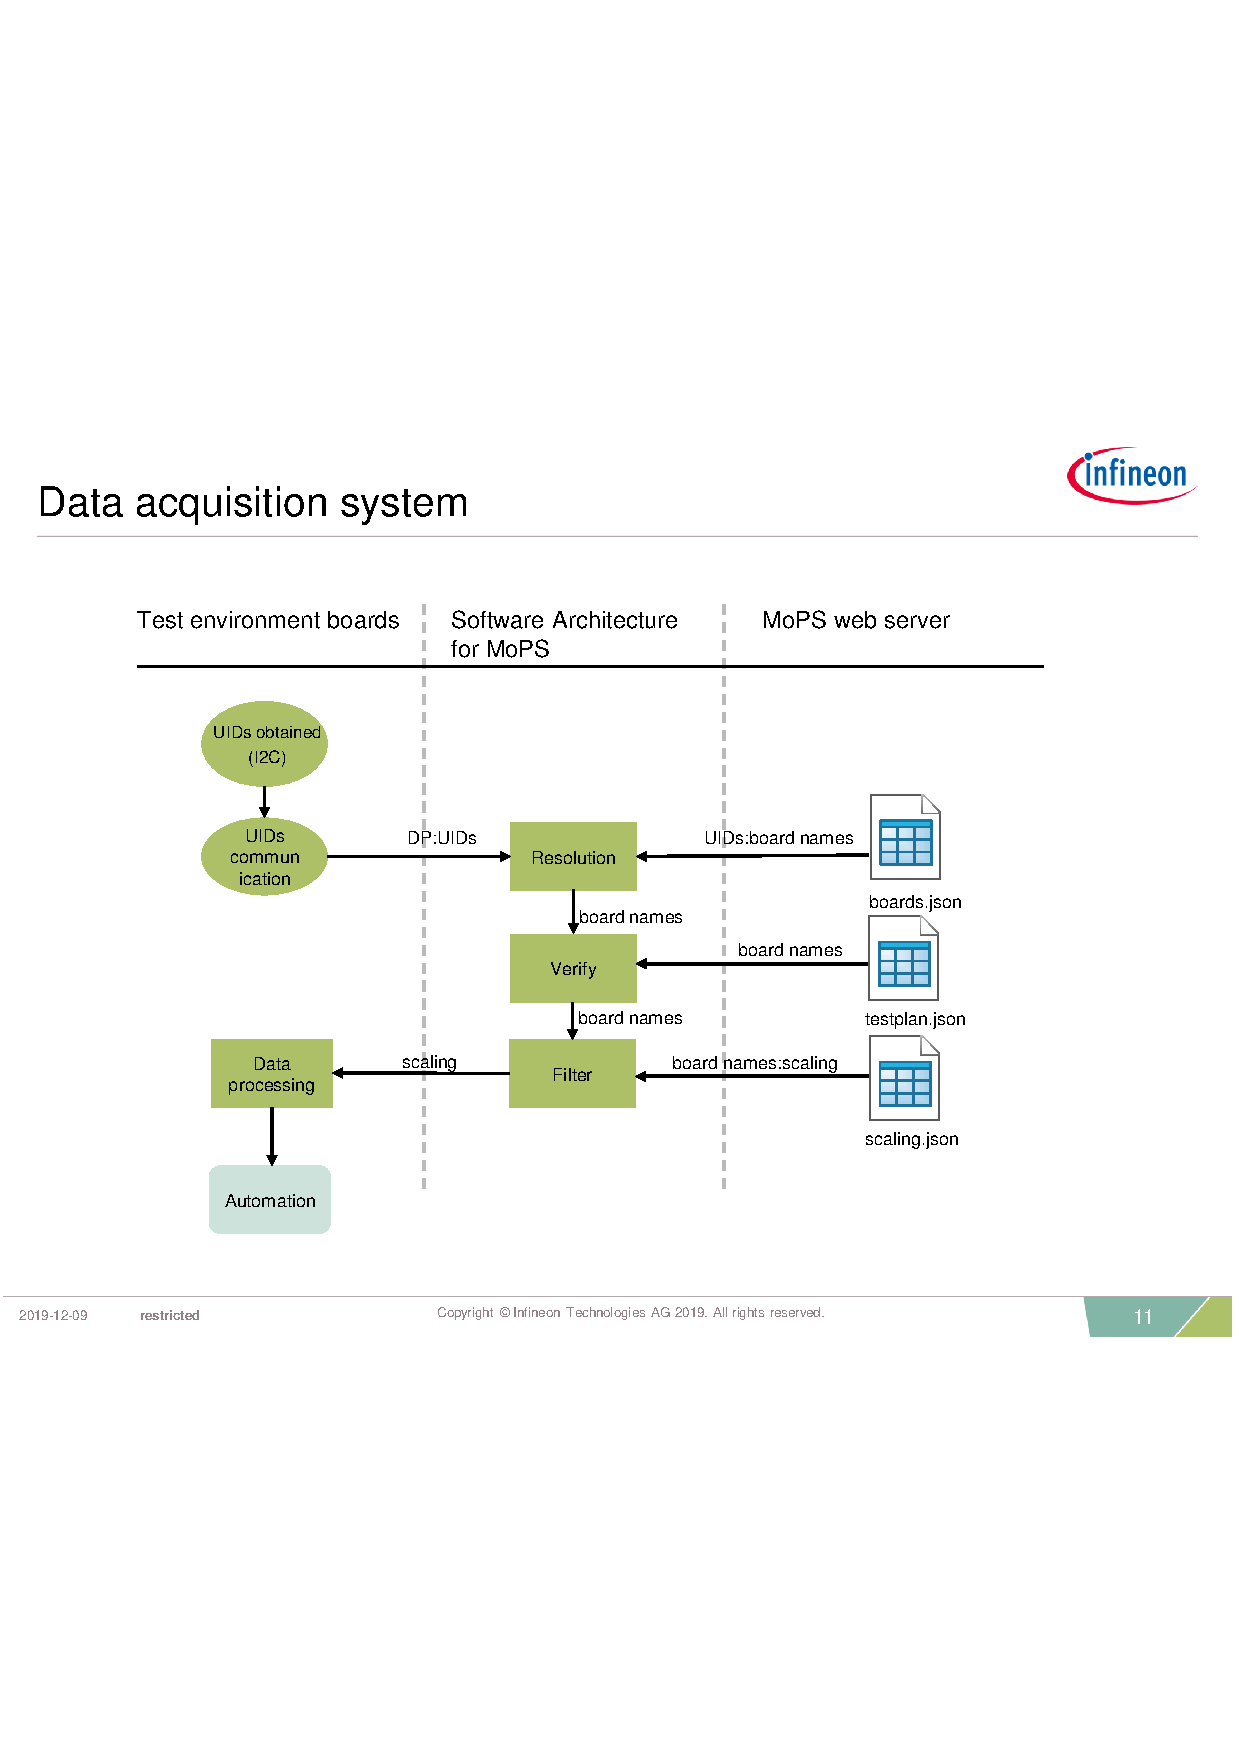
\includegraphics[trim=0 250 0 260, clip, width=160mm]{images/resolution.pdf}
		\caption{Resolution of board UIDs and scaling values communication}
		\label{fig:resolution}
\end{figure}
The board names that are fetched after the resolution of the board UIDs, are further authenticated with the board names that are present in the test plan. 
The board names that are present in the test plan are the hardware information provided by test engineers. 
Verification of boards are done in order to maintain consistency between the actual board connections and the test engineers selection of boards in the test plan. %In the perspective of this project, the board connections of Low Voltage MTS is as shown in the figure\cref{combination} and the respective test engineers hardware selection should be as shown in the ovenplan window(see Section \cref{TP}) of test plan.     
%Test engineers select the boards that are appropriate to the type of stress test that they are interested in conducting.
After the successful verification of board names in SAM, the verified board names are searched in the scaling connected \gls{LUT} to fetch the appropriate MicroMoPS channels and their scaling values.  

\subsection{Send the scaling values to MicroMoPS.}\label{sec:send}
The fetched communication channels and their corresponding scaling values are sent in queue as a string back to data processing system of MicroMoPS, using Ethernet communication.
The communication channels and their scaling values that are received at scaling related receiver handler of MicroMoPS are dynamically parsed to appropriately adjust the scaling values to the channels specific scaling variables (see \cref{lst:code_scaling}).
\subsection{Execute Low Voltage Test System}\label{sec:LowVoltage}
After successful adjustment of the scaling parameters in the MicroMoPS, the test sequence which is forwarded by SAM is executed on MicroMoPS. 
Finally, after all the above phases, the linear scaling mechanism and the Reverse Polish Notation get successfully integrated into the data processing system of MicroMoPS. 
The entire procedure of resolving the board UIDs supports to the automation of processing of analog measurements in MicroMoPS.
Measurements that are processed using linear scaling and Reverse Polish Notation are acquired at SAM and manipulated to retain the original values of analog measurements for any interpretation.
  